% start preamble -------------------------------------------------------------
\documentclass{article}
\usepackage{amsmath, amsthm, amssymb, amsfonts}
\usepackage{thmtools}
\usepackage{graphicx}
\usepackage{setspace}
\usepackage{geometry}
\usepackage{float}
\usepackage{hyperref}
\usepackage[utf8]{inputenc}
\usepackage[english]{babel}
\usepackage{framed}
\usepackage[dvipsnames]{xcolor}
\usepackage{tcolorbox}
\usepackage{ dsfont }
\usepackage[math]{cellspace}
\usepackage{ tipa }

\setlength\cellspacetoplimit{3pt}
\setlength\cellspacebottomlimit{3pt}
\colorlet{LightGray}{White!90!Periwinkle}
\colorlet{LightOrange}{Orange!15}
\colorlet{LightGreen}{Green!15}

\graphicspath{ {./pictures/} }

\newcommand{\HRule}[1]{\rule{\linewidth}{#1}}
\newcommand{\tab}{\qquad \qquad}
% end preamble -------------------------------------------------------------------

\begin{document}

% ------------------------------------------------------------------------------
% Cover Page and ToC
% ------------------------------------------------------------------------------

\title{ \normalsize \textsc{}
		\\ [2.0cm]
		\HRule{1.5pt} \\
		\LARGE \textbf{\uppercase{ Mathe 2 Hausübung Nr.2 }
        \HRule{2.0pt} \\ [0.6cm] \LARGE{ Sebastian Steitz, Hannes Albert } \vspace*{10\baselineskip}}
		}
\date{Juni 2023}
\author{\textbf{} \\
		Gruppe: 6\\
		Tutor: Zidane Bürmann }

\maketitle
\setlength\leftskip{1cm}

\section*{H10.1} 
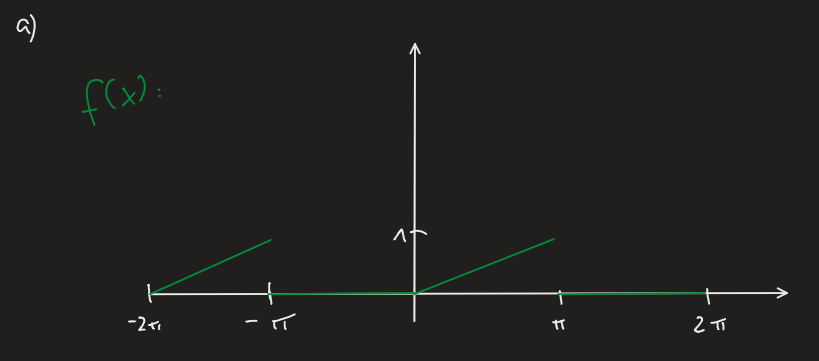
\includegraphics[scale=0.5]{ 1 } \\ 
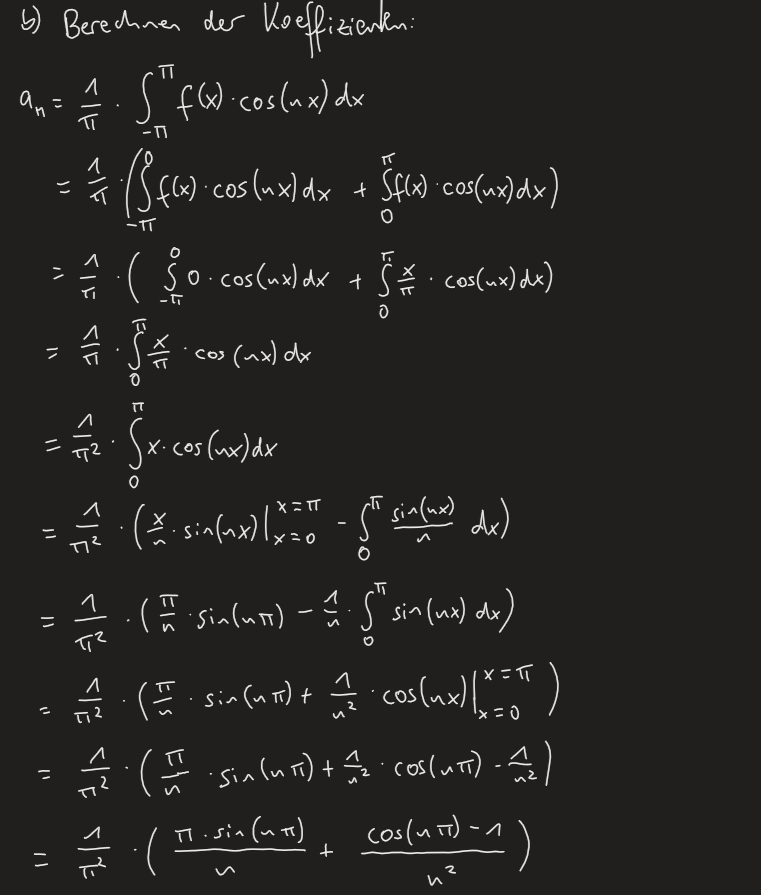
\includegraphics[scale=0.5]{ 2 } \\ 
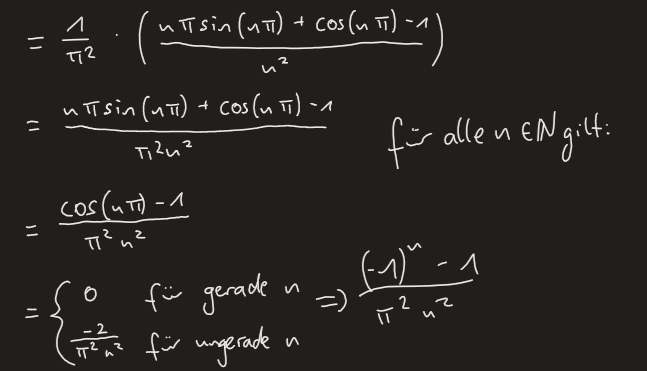
\includegraphics[scale=0.5]{ 3 } \\ 
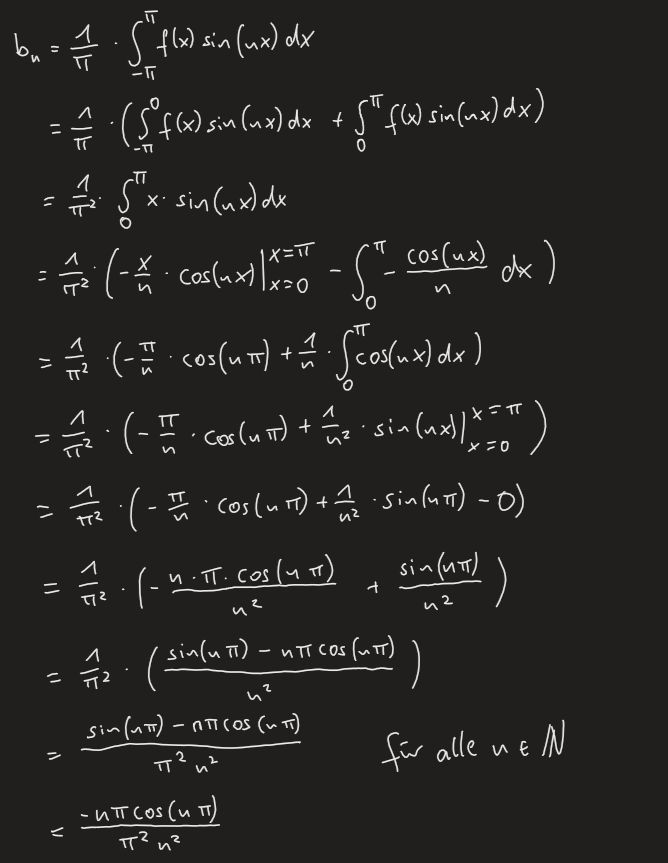
\includegraphics[scale=0.5]{ 4 } \\ 
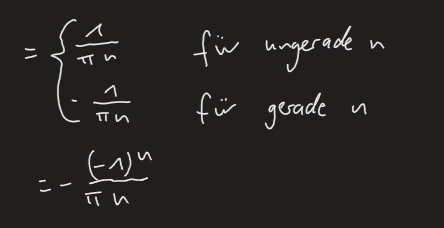
\includegraphics[scale=0.5]{ 5 } \\ 
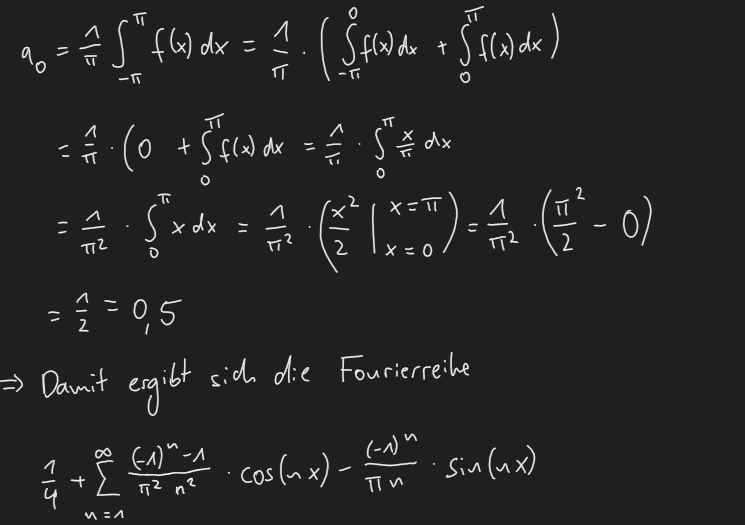
\includegraphics[scale=0.5]{ 6 } \\ 
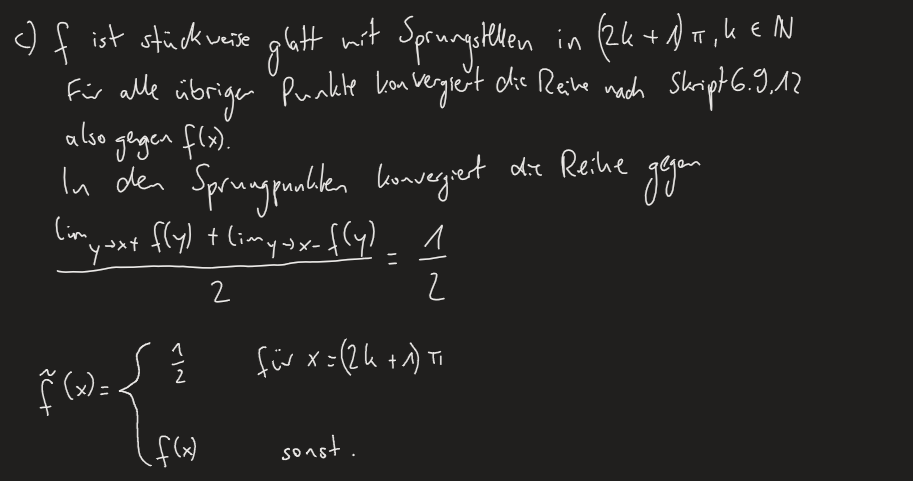
\includegraphics[scale=0.5]{ 7 } \\ 
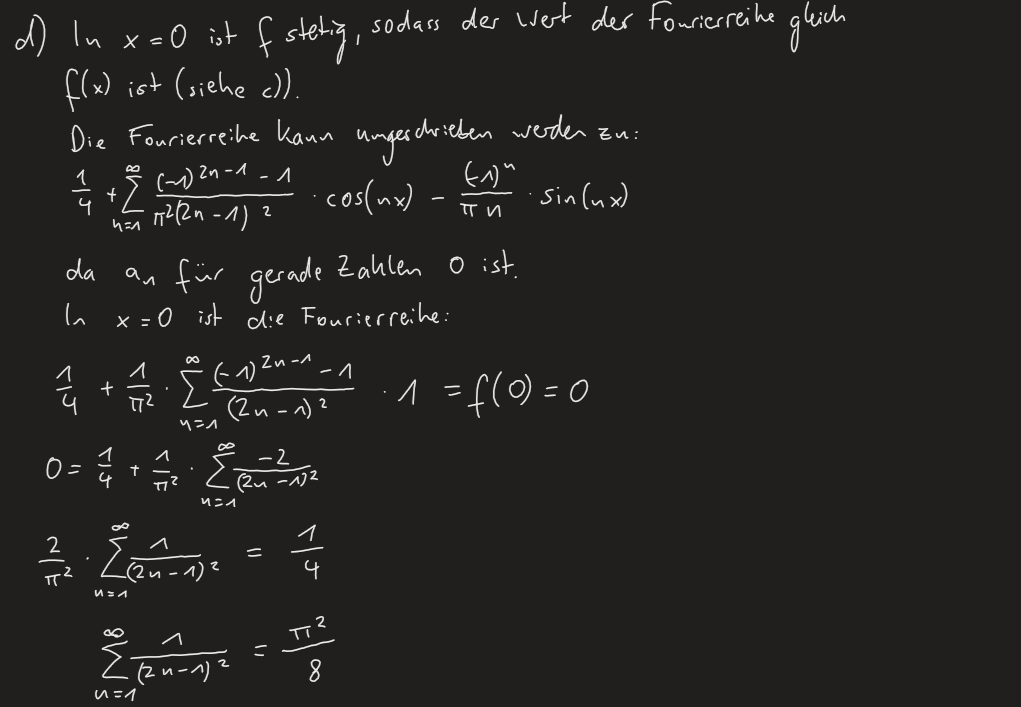
\includegraphics[scale=0.5]{ 8 }

\section*{H10.2}
\begin{align*}
    z(t) &= \frac{y(t)}{t} \\ 
    z'(t) &= y'(t) * \frac{1}{t} + y(t) * (- \frac{1}{t^2}) \\ 
          &= y'(t) * \frac{1}{t} - y(t) * \frac{1}{t^2} \\
          &= \frac{t * y'(t) - y(t)}{t^2}
\end{align*}

Nun lösen wir dies nach y'(t) auf:

\begin{align*}
    z'(t) &= \frac{t * y'(t) - y(t)}{t^2} \tab |  +\frac{y(t)}{t^2} -z'(t) \\ 
    \frac{y'(t)}{t} &= z'(t) + \frac{y(t)}{t^2} \tab |  * t \\
    y'(t) &= z'(t) * t + \frac{y(t)}{t} \\ 
    y'(t) &= t * z'(t) + z(t)
\end{align*}

Damit erhalten wir:
\begin{align*}
    y'(t) = z'(t) * t + z(t) &= (1 + z(t))^2 - z(t) \\ 
                             &= 1 + 2z(t) + z(t)^2 - z(t) \\ 
                             &= 1 + z(t) + z(t)^2 \tab | -z(t) \\ 
                      z'(t) * t &= z(t)^2 + 1 \tab | \frac{1}{t} \\ 
                      z'(t) &= \frac{z(t)^2 + 1}{t}
\end{align*}
Im weitern verwenden wir eine Schmierrechnung:
$\frac{dz}{1 + z^2} = \frac{dt}{t}$
\[
    \int_{}^{} \frac{1}{1 + z^2} \, dz = \int_{}^{} \frac{1}{t} \, dt = ln(t) + c \tab c \in \mathds{R}
\]
Somit erhalten wir für y(t) unter Verwendung des Tipps für das Anfangswertproblem:
\begin{align*}
    y(t) &= t * z(t) = t * tan(ln(t) + c) \\  
    y(1) &= 1 \\ 
    1 &= 1 * tan(c) \\ 
    c &= \frac{\pi}{4}
\end{align*}

\[
    \rightarrow y(t) = t * tan(ln(t) + 4) \tab t \in (e^{-\frac{3}{4}, e^{\pi}{4}})
\]

\noindent Da wir eine Schmierrechnung verwendet haben müssen wir noch einem mal eine Probe anstellen:
\begin{align*}
    y(1) &= 1 * tan(ln(1) + \frac{\pi}{4}) = 1 \\ 
    y'(t) &= \frac{t^2 * z'(t) + z(t)}{t} \\ 
          &= t * \frac{z(t)^2 + 1}{t} + \frac{t * tan(ln(t) + \frac{\pi}{4})}{t} \\ 
          &= (\frac{y(t)}{t})^2 + 1 + \frac{y(t)}{t} \\ 
          &= (\frac{y(t)}{t} + 1)^2 - 2 * y(t) + (y(t)) \\ 
          &= (\frac{y(t)}{t} + 1)^2 - y(t) 
\end{align*}
Damit sind wir fertig.
\end{document}

